\documentclass[10pt, xcolor=dvipsnames]{beamer}
%\documentclass[10pt, xcolor=dvipsnames,notes=only]{beamer}
%\mode<presentation>
%{
\usetheme{Goettingen}
%\setbeamercovered{transparent}
%} 
\usefonttheme{professionalfonts}
%\usecolortheme{beaver}

\usepackage{setspace}
\usepackage[english]{babel}
\usepackage[latin1]{inputenc}
\usepackage{times}
\usepackage[T1]{fontenc}
\usepackage{color}
\usepackage{graphicx}
\usepackage{amssymb}
\usepackage{amsthm}
\usepackage{bm}
\usepackage{rotating}
\usepackage{ccaption}
\usepackage{booktabs}
\usepackage{lscape}
\usepackage{colortbl}
\usepackage{arydshln}
\usepackage{tabularx}
\usepackage{graphics}
\usepackage{epstopdf}

\setbeamertemplate{navigation symbols}{}
\setbeamertemplate{items}[balls]

\newenvironment{changemargin}[2]{%
  \begin{list}{}{%
    \setlength{\topsep}{0pt}%
    \setlength{\leftmargin}{#1}%
    \setlength{\rightmargin}{#2}%
    \setlength{\listparindent}{\parindent}%
    \setlength{\itemindent}{\parindent}%
    \setlength{\parsep}{\parskip}%
  }%
  \item[]}{\end{list}}

\setbeamercolor{block title}{fg=white, bg=teal}
\setbeamercolor{block body}{bg=teal!25}

\author[]{Chad Jones and Dietrich Vollrath}
\institute[Intro Growth]{Introduction to Economic Growth}
\date[]{}


\title[Social infrastructure]{Social infrastructure and long-run growth}


\begin{document}
\maketitle

\section{An investment problem}
\begin{frame}{Rich and poor}
We have several reasons why countries could be rich or poor:
\begin{itemize}
	\item Physical capital formation ($s_I$)
	\item Human capital ($h$), skills and diffusion
	\item R\&D ($s_R$)
	\item Population growth ($g_L$), both negative and positive
	\item Trade and diffusion of innovations
	\item Mis-allocations of factors
\end{itemize}
\end{frame}

\begin{frame}{Investments}
Could conceive of each in terms of making a choice on how to use resources:
\begin{itemize}
	\item Physical capital: use $L$, $K$ to build more capital
	\item Human capital: use $L$, $K$ to educate workers
	\item R\&D: use $L$, $K$ to innovate
	\item Population growth: use $L$, $K$ to create more people
	\item Trade/diffusion: use $L$, $K$ to make trade or adoption possible 
	\item Misallocation: use $L$, $K$ in better/worse ways
\end{itemize}
\end{frame}

\begin{frame}{$F$ and $V$}
A general decision process would be to evaluate the costs ($F$) against benefits ($V$). Think of costs $F$:
\begin{itemize}
	\item Lost consumption while investing in capital goods
	\item Time spent in school
	\item Time spent by researchers/innovators
	\item Time spent raising a family and not working (or working in amenable positions)
	\item Capital and labor spent building physical and legal structure to import/adopt
	\item Lost output of good $i$ if you push factors to good $j$
\end{itemize}
\end{frame}

\begin{frame}{$F$ and $V$}
Think of benefits $V$:
\begin{itemize}
	\item Continued use of the capital good over time
	\item Application of skills learned over time
	\item Innovation that can be used over time (and shared)
	\item More people available to work/innovate/invest over time
	\item New varieties available over time
	\item Higher overall output
\end{itemize}
\end{frame}

\begin{frame}{Now and later}
A lot of the comparison of $F$ and $V$ comes down to
\begin{itemize}
	\item Incurring a cost, $F$, now
	\item For benefits, $V$, that accrue in the future
\end{itemize}
In the end you make the investment/innovate/educate/reform if $V > F$
\end{frame}

\begin{frame}{Higher $F$}
If you make $F$ higher, you make fewer investments worthwhile:
\begin{itemize}
	\item Bribes, corruption
	\item Procedures/regulations
	\item Crime/safety
\end{itemize}
Note that you might \textit{want} to slow down some investments (e.g. narcotic production) via these routes.
\end{frame}

\begin{frame}{Higher $V$}
The value of a project/investment is something like
\begin{equation}
	V_t = \frac{\pi_t}{r-g_{\pi}+\rho}, \nonumber
\end{equation}
where $\pi_t$ is the initial profits you can make, $r$ is discount on the future, and $g_{\pi}$ is how fast profits grow. $\rho$ is a chance you lose rights to that project for whatever reason. 
\begin{itemize}
	\item If policies (market structure, taxes) lower $\pi_t$, less value
	\item If property rights over project are insecure, $\rho$ is high, less value
	\item If \textit{others} don't value future, $r$ is high, less value
	\item If \textit{others} don't invest, $g_{\pi}$ is low, less value
\end{itemize}
Lump a lot of this together as ``social infrastructure'' and whether it supports high $V$ and low $F$
\end{frame}

\section{Raw indicators}
\begin{frame}{Social infrastructure}
No clear way to measure this. World Bank collects measures of things like:
\begin{itemize}
	\item Accountability of political leaders
	\item Political stability
	\item Government effectiveness
	\item Regulatory quality
	\item Rule of law
	\item Control of corruption
\end{itemize}
These are often measured via survey of perceptions. We take average of these six to measure ``social infrastructure''
\end{frame}

\begin{frame}{Physical capital}
\begin{center}
\includegraphics[height=3in]{../Figures/fig-ch8-fig1.eps}
\end{center}
\end{frame}

\begin{frame}{Human capital}
\begin{center}
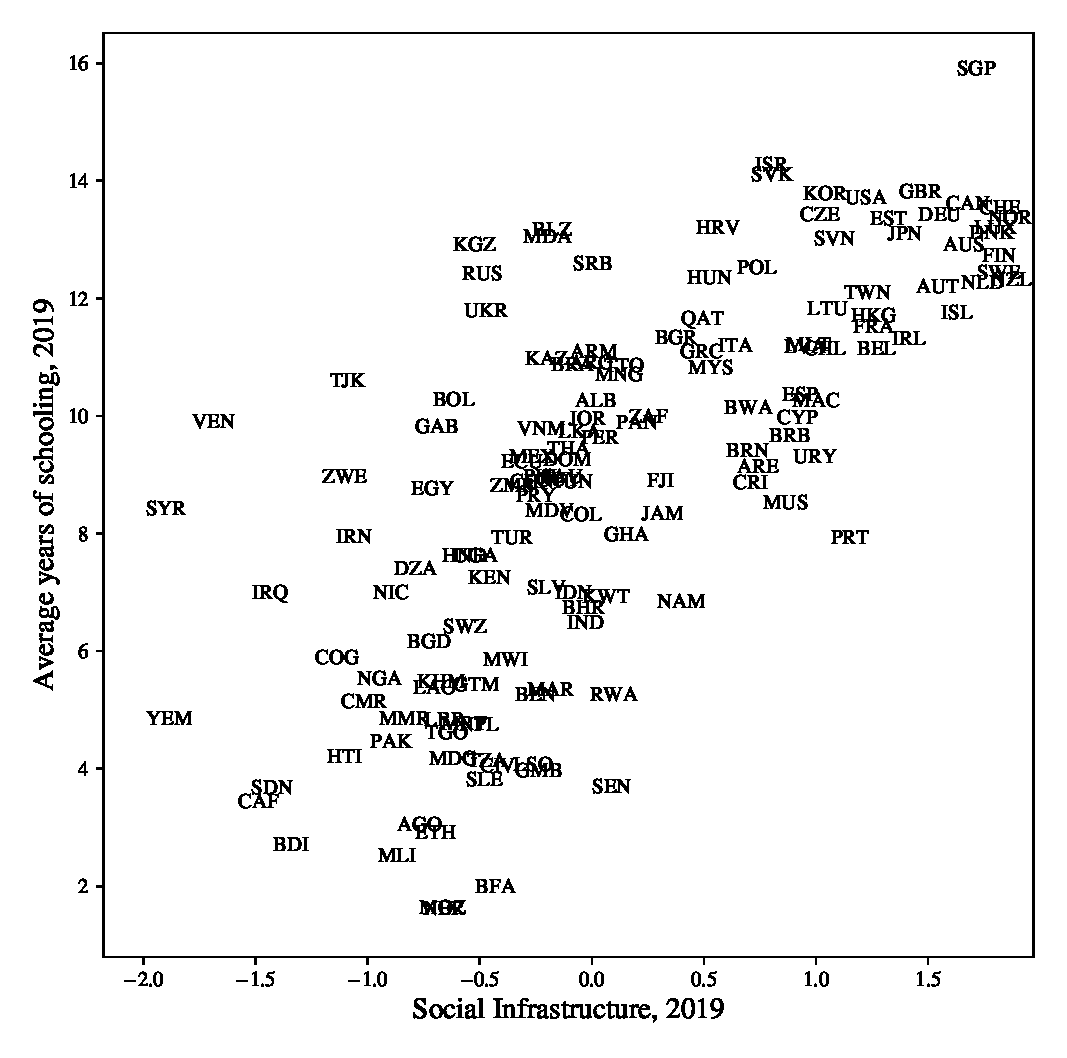
\includegraphics[height=3in]{../Figures/fig-ch8-fig2.eps}
\end{center}
\end{frame}

\begin{frame}{Productivity}
\begin{center}
\includegraphics[height=3in]{../Figures/fig-ch8-fig3.eps}
\end{center}
\end{frame}

\begin{frame}{Causality}
We don't know if this is causal
\begin{itemize}
	\item Higher capital accumulation could lead to higher GDP per capita, which allows places to invest in social infrastructure: maybe this goes the other way
	\item Individual studies point towards social infrastructure determining these outcomes
	\item Specific historical instances (e.g. North/South Korea) are examples where differences in social infrastructure seem to determine level of GDP per capita
\end{itemize}
\end{frame}

\section{Choosing underdevelopment}
\begin{frame}{Why not fix this?}
Things that raise $F$ and lower $V$ are subject to change. Why don't poor countries
\begin{itemize}
	\item Lower regulatory burdens
	\item Eliminate corruption
	\item Assure property rights
	\item Support more education
	\item Create more effective governments
\end{itemize}
The benefit is that this would raise GDP. What's stopping them?
\end{frame}

\begin{frame}{Someone benefits}
Each individual case is unique. General story is something like
\begin{itemize}
	\item \textit{Someone} benefits from current structure (e.g. a bribe-taker)
	\item Improving social infrastructure involves those people losing
	\item You could promise to give losers a slice of the increased GDP
	\item But those promises may not be credible
	\item So no one can or will make that deal
\end{itemize}
\end{frame}

\end{document}